\documentclass[aspectratio=169,10pt]{beamer}
\usepackage{booktabs}
\usepackage{tikz}

% ---------- UniPD template look (red band + logo), default LaTeX fonts ----------
\definecolor{pdred}{HTML}{B3071B}
\setbeamercolor{background canvas}{bg=white}
\setbeamercolor{frametitle}{fg=black,bg=white}
\setbeamercolor{structure}{fg=pdred}
\setbeamercolor{itemize item}{fg=pdred}
\setbeamercolor{itemize subitem}{fg=pdred}
\setbeamercolor{block title}{bg=pdred,fg=white}
\setbeamercolor{block body}{bg=pdred!6,fg=black}
\setbeamertemplate{navigation symbols}{}
\setbeamertemplate{itemize item}[circle]
\setbeamerfont{frametitle}{series=\bfseries,size=\large}
\setbeamerfont{block title}{size=\small}
\setbeamerfont{block body}{size=\small}

\setbeamertemplate{background}{%
  \begin{tikzpicture}[remember picture,overlay]
    \fill[pdred] (current page.north west) rectangle ([yshift=-14.9mm]current page.north east);
    \node[anchor=north west,inner sep=0] at ([xshift=4.7mm,yshift=-2.3mm]current page.north west)
      {
\includegraphics[width=37.5mm]{figs/unipd_logo.png}};
  \end{tikzpicture}}
\setbeamertemplate{frametitle}{%
  \vskip 1.2mm\insertframetitle\par}
\addtobeamertemplate{frametitle}{}{\vskip-1mm}
\setbeamertemplate{headline}{\vspace*{14.9mm}}
\setbeamertemplate{footline}{%
  \hfill{\tiny\color{gray}\insertframenumber\hspace{4mm}}\vskip2mm}
\setbeamersize{text margin left=6mm,text margin right=6mm}
\newcommand{\alignednoiseplot}[1]{%
  \begin{tikzpicture}[remember picture,overlay]
    \node[anchor=north,inner sep=0] at ([xshift=0.333\paperwidth,yshift=-0.37\paperheight]current page.north west)
      {\includegraphics[width=0.60\paperwidth]{#1}};
  \end{tikzpicture}}

\newcommand{\figorbox}[4]{% file, width, height, caption if the file is missing
  \IfFileExists{#1}{\includegraphics[width=#2]{#1}}{%
    \fcolorbox{pdred}{pdred!5}{\parbox[c][#3][c]{\dimexpr#2-2\fboxsep-2\fboxrule}{\centering\small\color{pdred}[#4]}}}}

\title{Lab 1: 4th-order elliptic low-pass filter}
\subtitle{Integrated Circuits for Signal Processing}
\author{Lorenzo Tomba, Peter Collavino, Gregorio Massella, Alveena Magsi}
\date{2 November 2026}

\begin{document}

% ---------- 1. Title ----------
\begingroup
\setbeamertemplate{background}{%
  \begin{tikzpicture}[remember picture,overlay]
    \fill[pdred] (current page.south west) rectangle (current page.north east);
    \node[anchor=north] at ([yshift=-14mm]current page.north)
      {
\includegraphics[width=95mm]{figs/unipd_logo.png}};
  \end{tikzpicture}}
\setbeamertemplate{headline}{}
\setbeamertemplate{footline}{}
\begin{frame}[plain]
  \vspace*{34mm}
  \begin{center}
    {\color{white}\Large Lab 1: 4th-order elliptic low-pass filter\\[1.5mm]
     \normalsize Integrated Circuits for Signal Processing\\[3mm]
     \small Lorenzo Tomba 2188353, Peter Collavino 2188355\\ Gregorio Massella 2165994, Alveena Magsi 2194853\\[2mm] 2 November 2026}
  \end{center}
\end{frame}
\endgroup

% ---------- 2. Specs ----------
\begin{frame}{Matlab Mathematical Result \& Specifications}
\begin{columns}[T,onlytextwidth]
\begin{column}{0.66\textwidth}
  \centering
  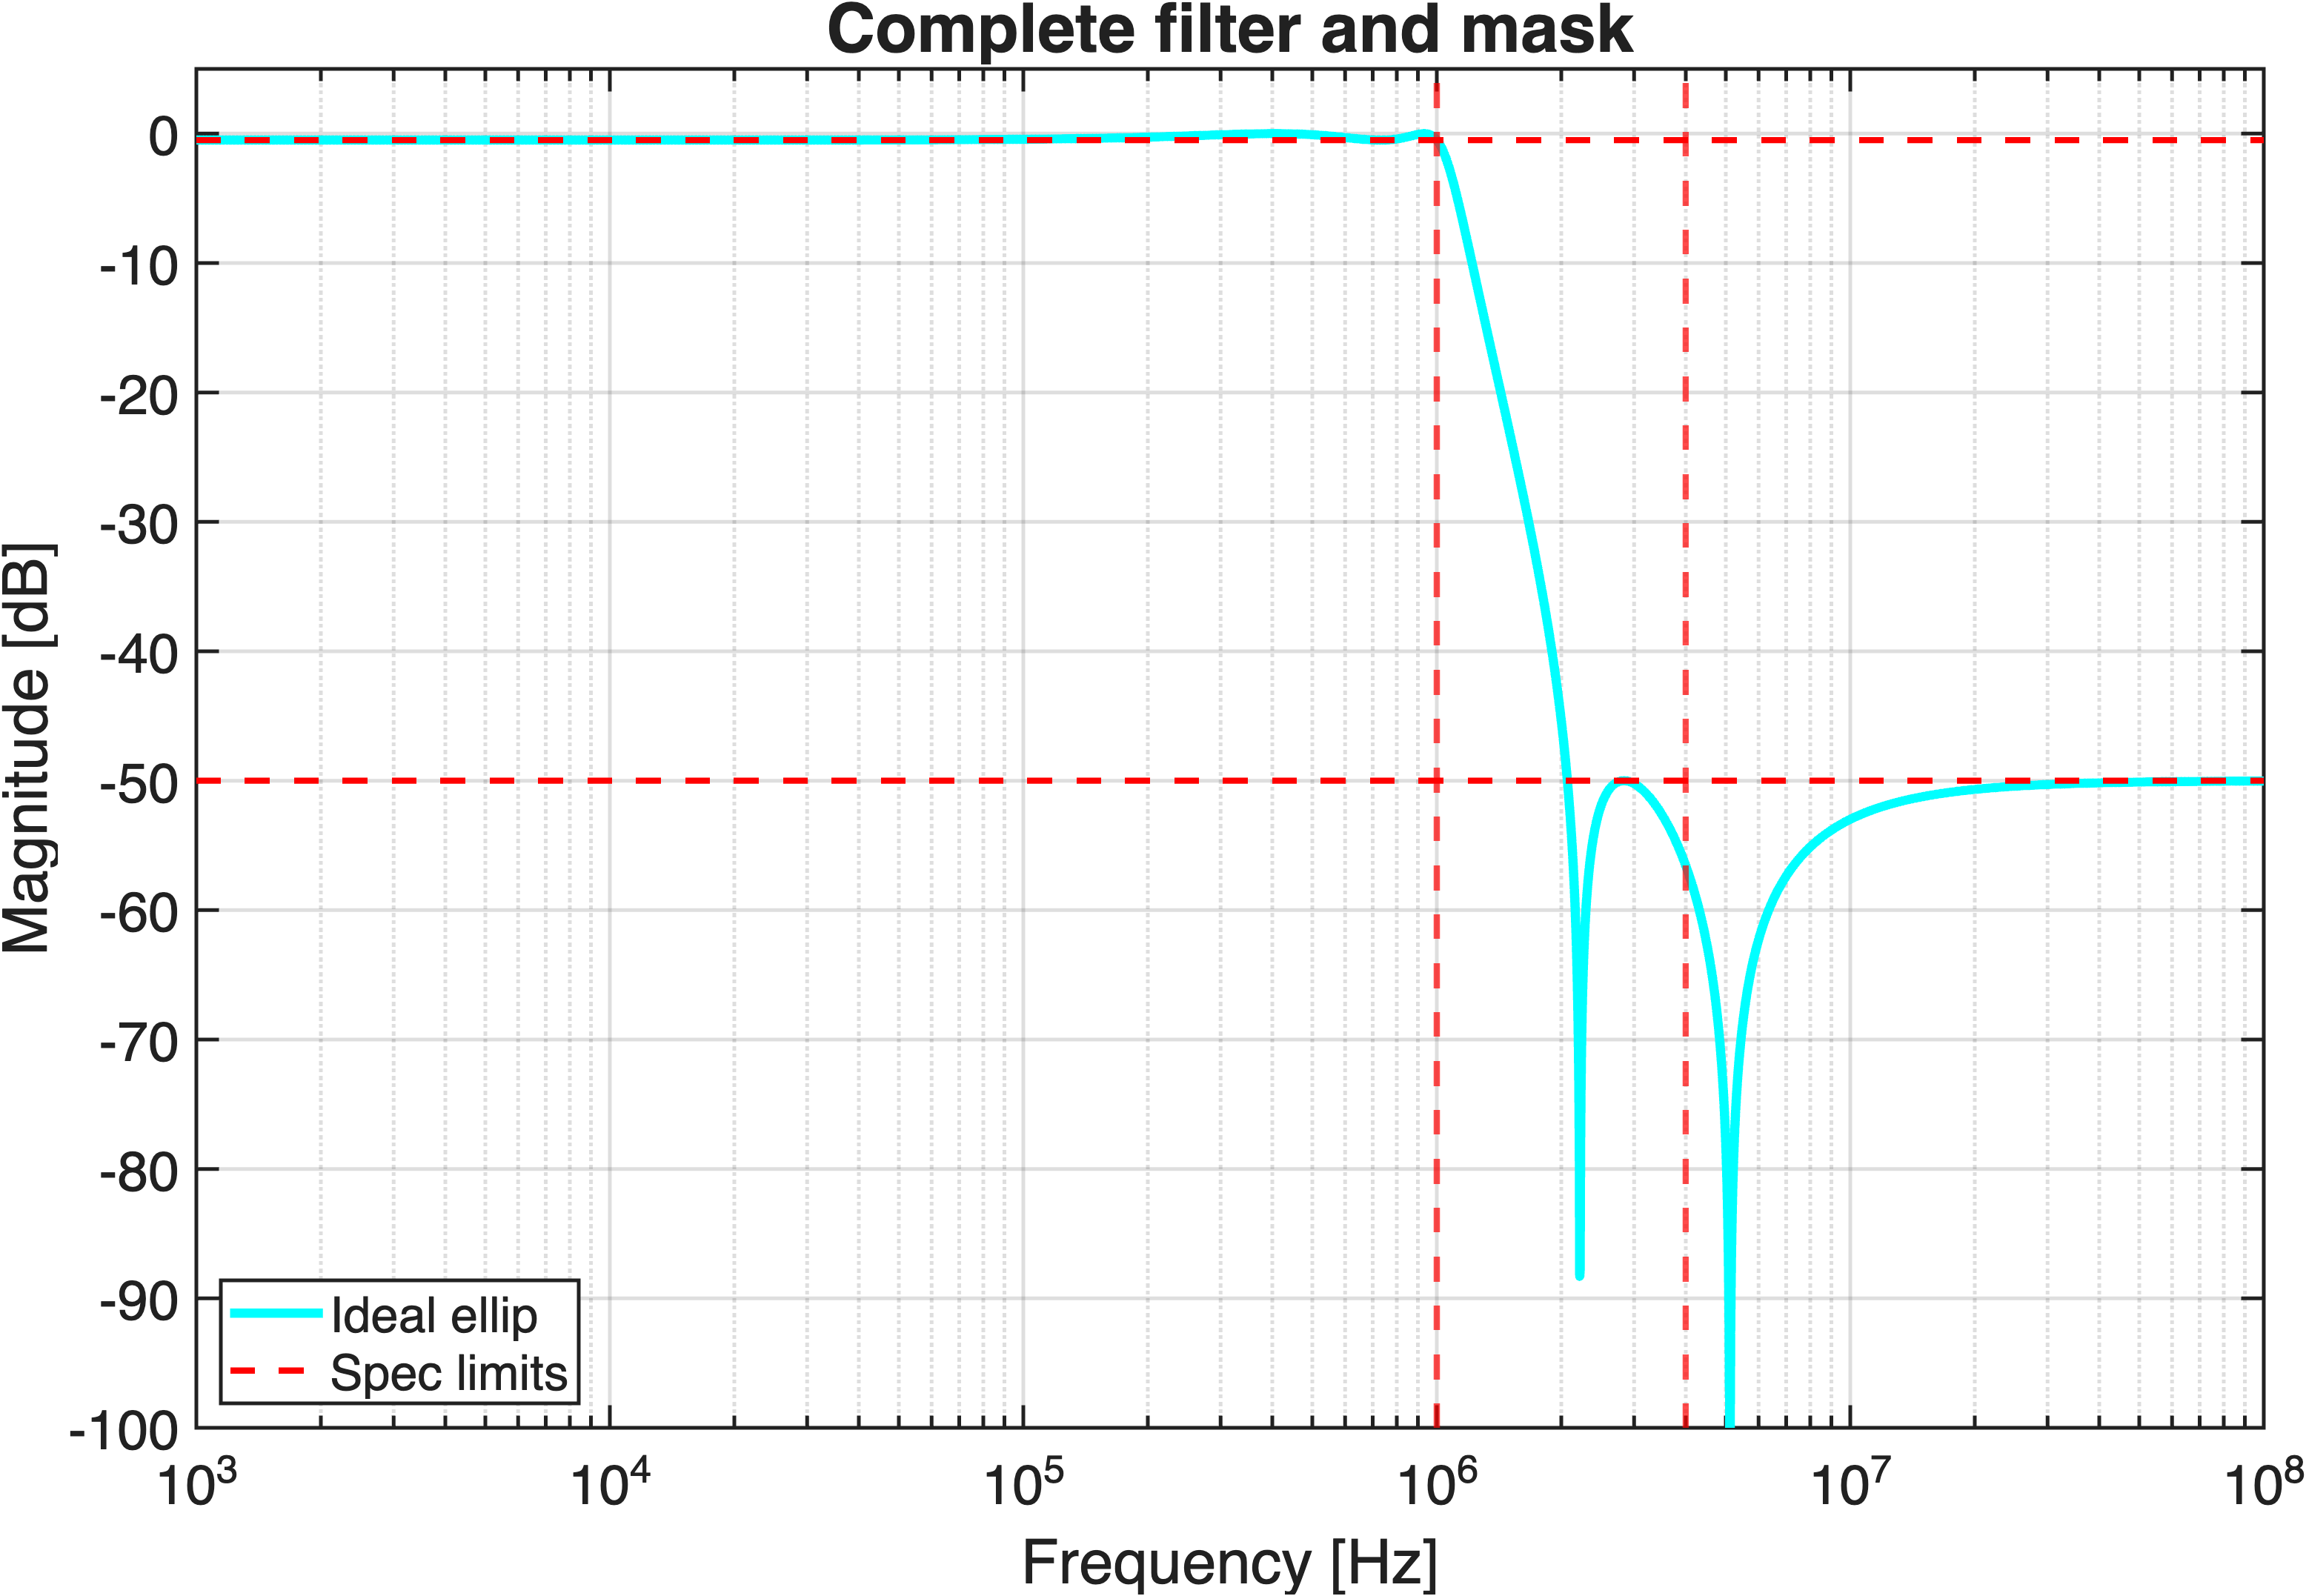
\includegraphics[width=\linewidth,height=0.84\textheight,keepaspectratio]{figs/filtro_completo.png}
\end{column}
\begin{column}{0.32\textwidth}
  \small
  \begin{itemize}\setlength\itemsep{1.5mm}
    \item 4th-order low-pass elliptic filter, ellipord gives minimumm order $N=3$
    \item Pass band edge $f_p=1$ MHz, stop pand edge $f_s=4$ MHz
    \item In-band ripple $\le 0.5$ dB, stop-band attenuation $\ge 50$ dB
    \item Output noise $<120\ \mu$V$_{\rm rms}$
  \end{itemize}
\end{column}
\end{columns}
\end{frame}

% ---------- 3. Pass band and stop band zoom ----------
\begin{frame}{Pass Band \& Stop Band Zoom}
\begin{columns}[T,onlytextwidth]
\begin{column}{0.5\textwidth}
  \centering
  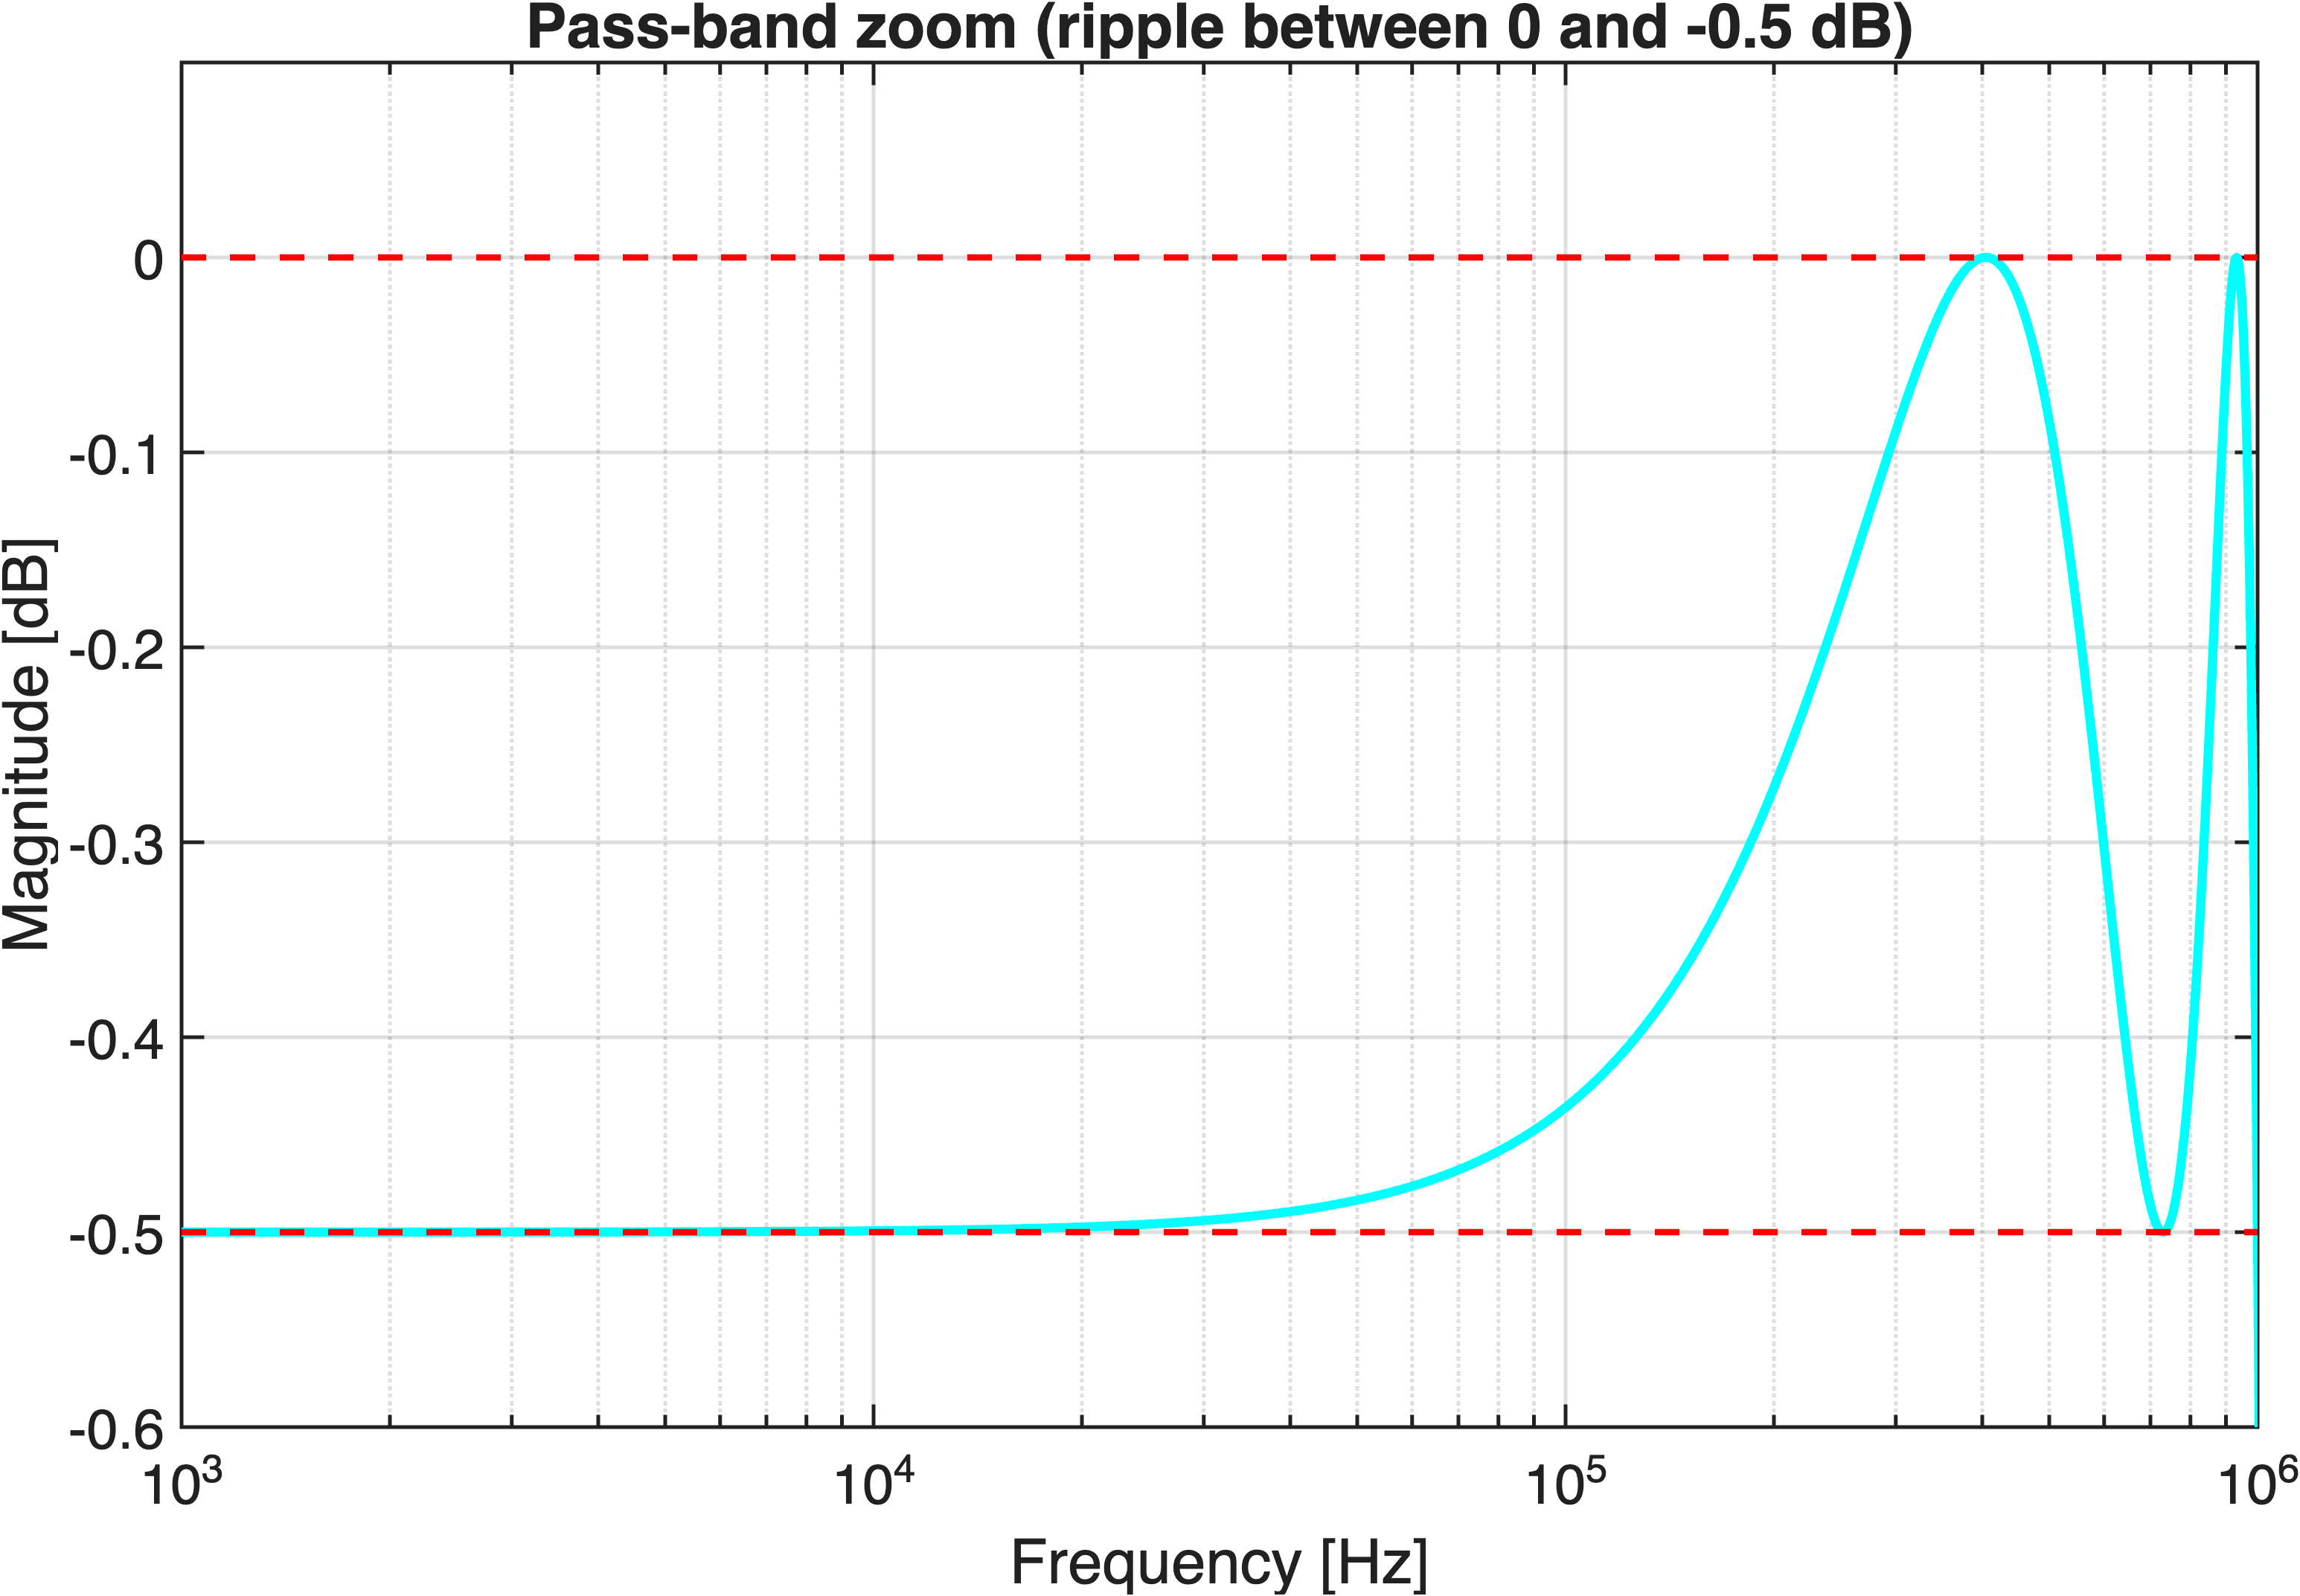
\includegraphics[width=\linewidth,height=0.78\textheight,keepaspectratio]{figs/passband_zoom.png}
\end{column}
\begin{column}{0.5\textwidth}
  \centering
  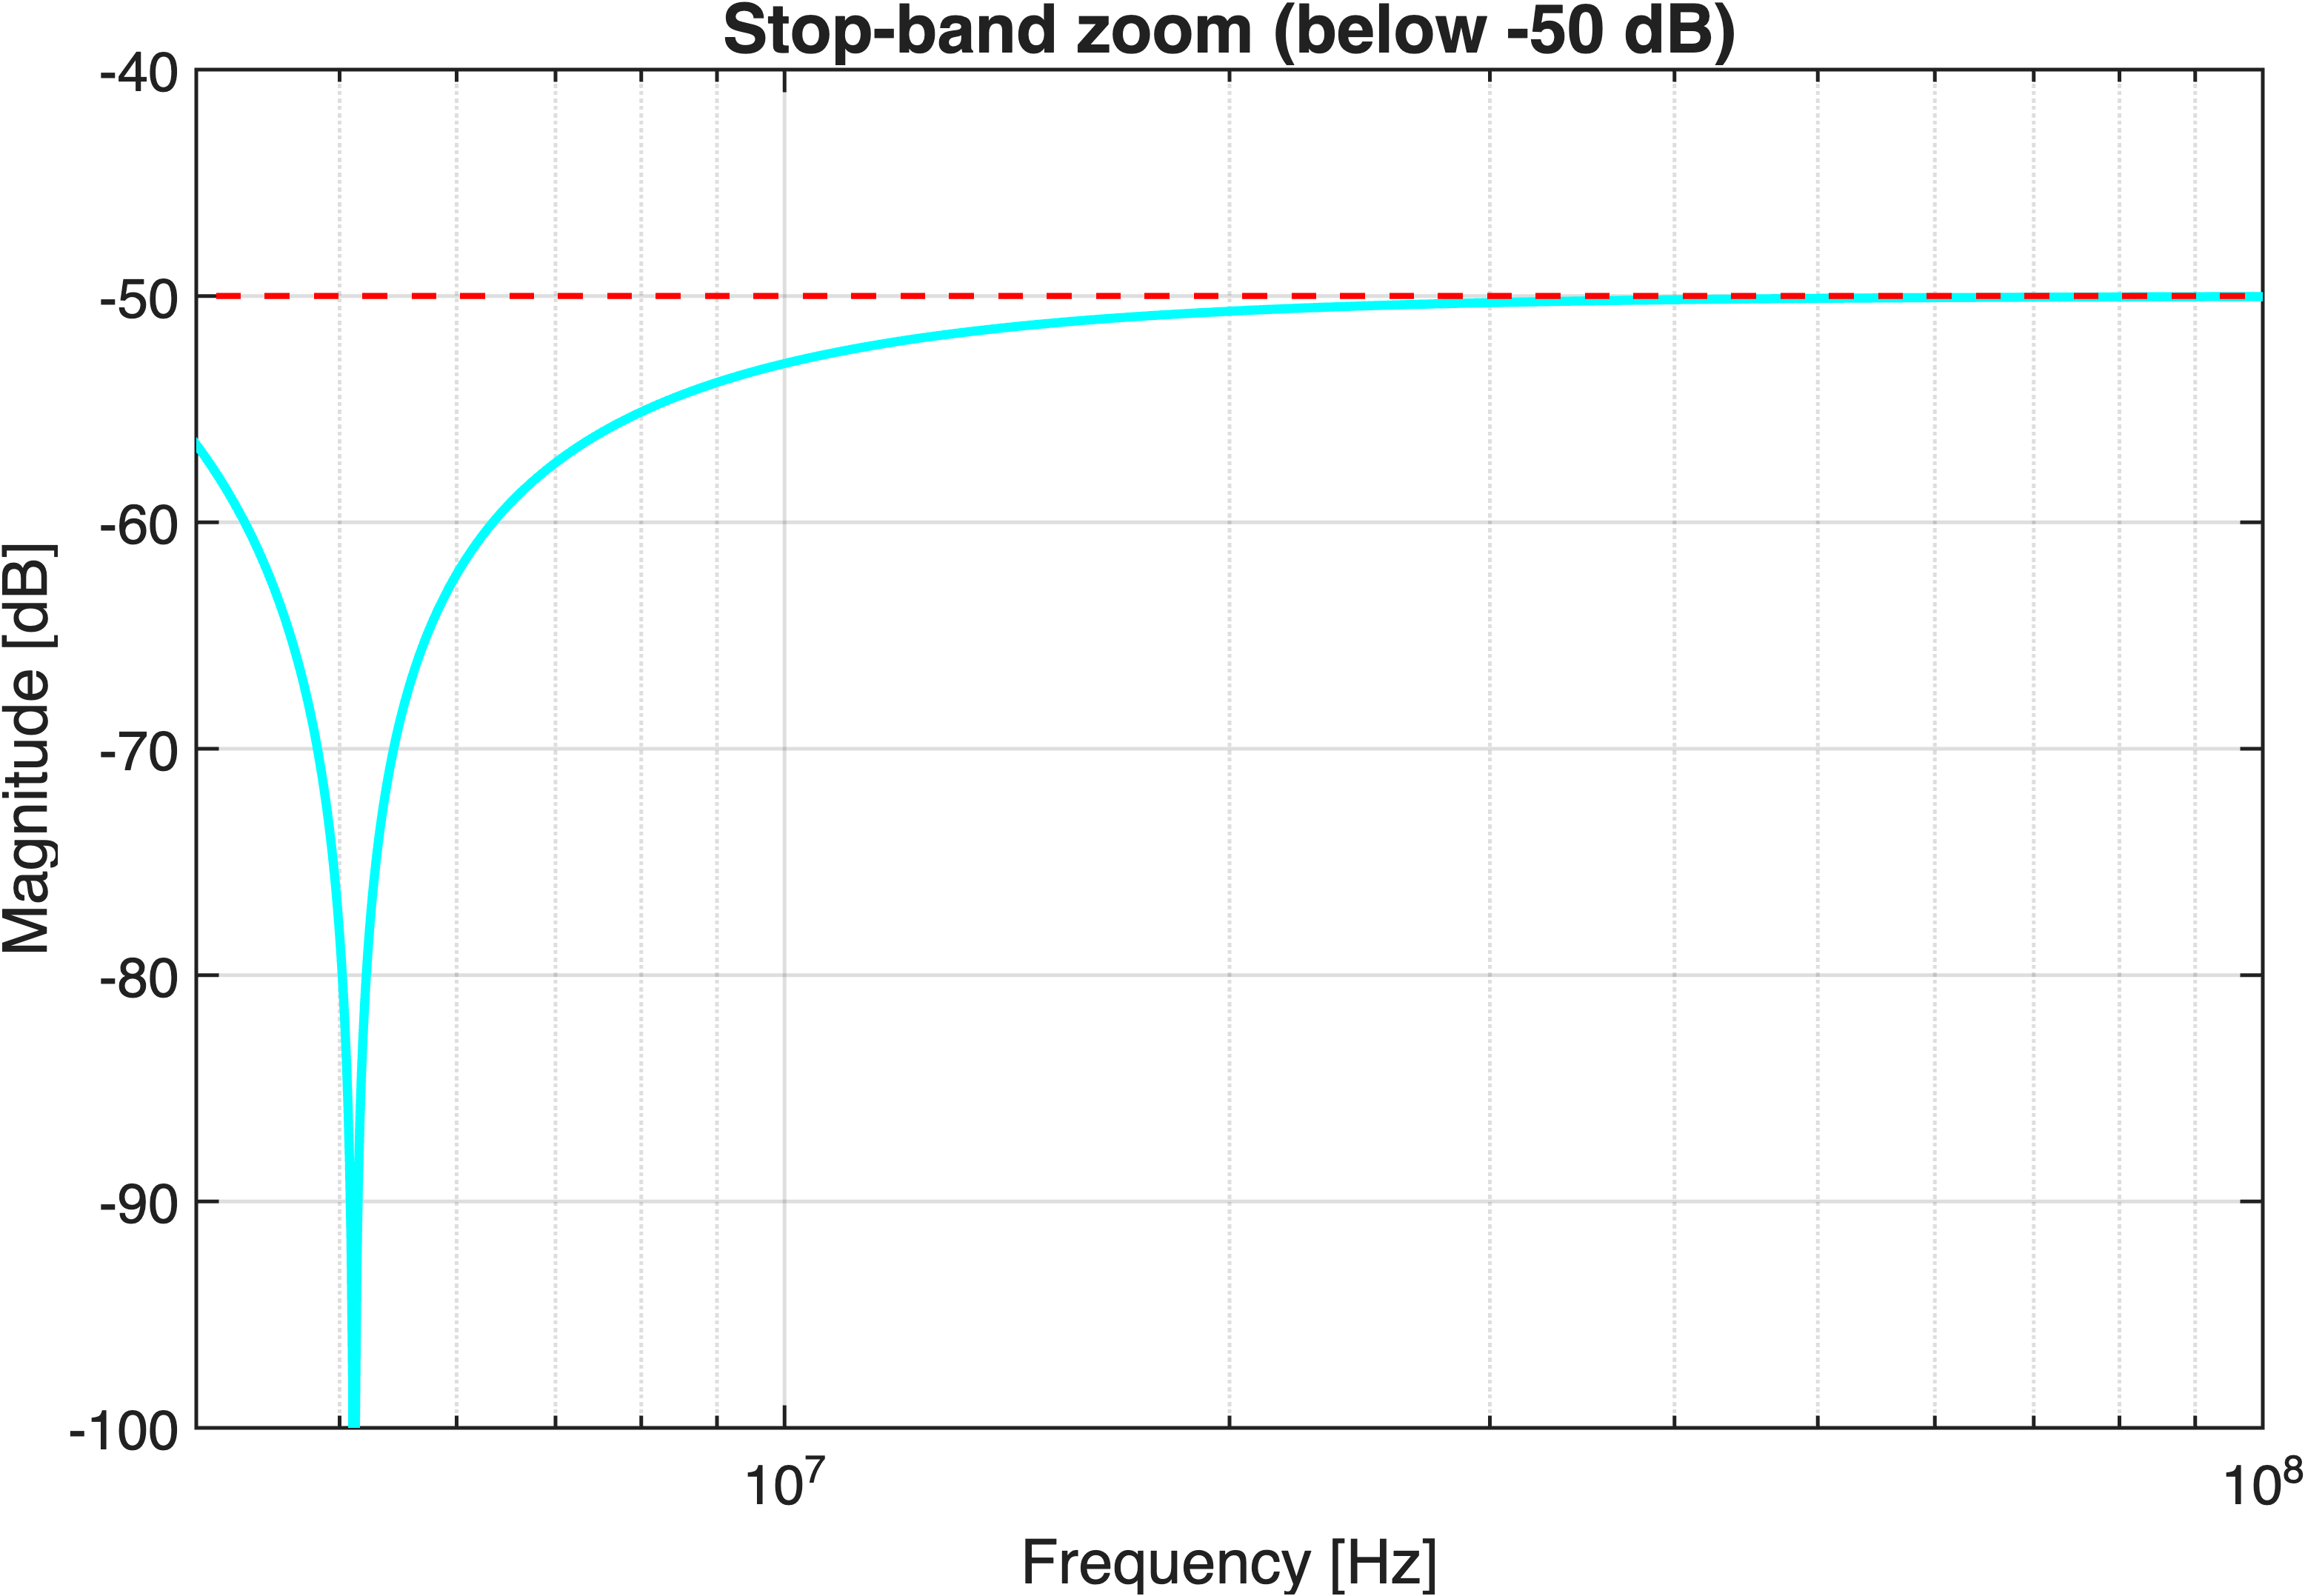
\includegraphics[width=\linewidth,height=0.78\textheight,keepaspectratio]{figs/stopband_zoom.png}
\end{column}
\end{columns}
\end{frame}

% ---------- 4. Biquad decomposition ----------
\begin{frame}{Biquad Decomposition}
\begin{columns}[T,onlytextwidth]
\begin{column}{0.64\textwidth}
  \small
  \begin{itemize}\setlength\itemsep{2mm}
    \item The overall filter transfer function can be decomposed into two separate second-order transfer functions.
    \item For each transfer function, we determine $k_0$, $k_1$, $k_2$, $Q$, and $\omega_0$. Biquad 1 has the lower $Q$ and comes first in the cascade, while Biquad 2 has higher Q and all the DC gain of the total transfer function
  \end{itemize}
  \vspace{4mm}
  \centering
  \resizebox{0.5\linewidth}{!}{$\displaystyle H(s)=\frac{k_2 s^2+k_1 s+k_0}{\dfrac{s^2}{\omega_0^2}+\dfrac{s}{Q\omega_0}+1}$}
\end{column}
\begin{column}{0.34\textwidth}
  \scriptsize
  \centering
  \setlength{\tabcolsep}{5pt}
  \textbf{Biquad 1}\par\vspace{1mm}
  \begin{tabular}{lc}
    \toprule
    Parameter & Value \\
    \midrule
    $\omega_0$ [rad/s] & $4.0039\times10^6$ \\
    $Q$ & $7.2264\times10^{-1}$ \\
    $k_0$ & $1.0000$ \\
    $k_1$ & $0.0000$ \\
    $k_2$ & $9.6813\times10^{-16}$ \\
    \bottomrule
  \end{tabular}

  \vspace{2mm}
  \textbf{Biquad 2}\par\vspace{1mm}
  \begin{tabular}{lc}
    \toprule
    Parameter & Value \\
    \midrule
    $\omega_0$ [rad/s] & $6.4771\times10^6$ \\
    $Q$ & $3.3831$ \\
    $k_0$ & $9.4406\times10^{-1}$ \\
    $k_1$ & $0.0000$ \\
    $k_2$ & $4.8566\times10^{-15}$ \\
    \bottomrule
  \end{tabular}
\end{column}
\end{columns}
\end{frame}

% ---------- 5. Component sizing and noise ----------
\begin{frame}{Component Sizing from the Noise Specification}
\begin{columns}[T,onlytextwidth]
\begin{column}{0.54\textwidth}
  \small
  \begin{itemize}\setlength\itemsep{1.5mm}
    \item The extracted parameters constrain the RC time constants. Component values must also meet the noise limit; deriving each noise-source-to-output transfer function is a long procedure, so we use a simpler estimate.
    \item Output noise power scales as $16kT/C$. With equal capacitors, a noise check lets us rescale all capacitances proportionally to the noise limit of the specifications.
  \end{itemize}
  \vspace{1mm}
  \[
    C_a=C_b=16\cdot\frac{kT}{V_{\mathrm{noise,RMS}}^2}\simeq 4.6\,\mathrm{pF}
  \]
\end{column}
\begin{column}{0.42\textwidth}
  \scriptsize
  \centering
  \setlength{\tabcolsep}{5pt}
  \textbf{Biquad 1}\par\vspace{1mm}
  \begin{tabular}{lcc}
    \toprule
    Component & Initial & After noise check \\
    \midrule
    $C_a=C_b$ & 4.6 pF & 9.2 pF \\
    $R_1$ & 39.2358 k$\Omega$ & 19.6179 k$\Omega$ \\
    $R_3$ & 54.2948 k$\Omega$ & 27.1474 k$\Omega$ \\
    $R_4$ & 54.2948 k$\Omega$ & 27.1474 k$\Omega$ \\
    $R_5$ & $-54.2948$ k$\Omega$ & $-27.1474$ k$\Omega$ \\
    $C_4$ & $-0.0714$ pF & $-0.1428$ pF \\
    \bottomrule
  \end{tabular}

  \vspace{1mm}
  \textbf{Biquad 2}\par\vspace{1mm}
  \begin{tabular}{lcc}
    \toprule
    Component & Initial & After noise check \\
    \midrule
    $C_a=C_b$ & 4.6 pF & 9.2 pF \\
    $R_1$ & 113.5463 k$\Omega$ & 56.7732 k$\Omega$ \\
    $R_3$ & 33.5629 k$\Omega$ & 16.7814 k$\Omega$ \\
    $R_4$ & 35.5516 k$\Omega$ & 17.7758 k$\Omega$ \\
    $R_5$ & $-33.5629$ k$\Omega$ & $-16.7814$ k$\Omega$ \\
    $C_4$ & $-0.9372$ pF & $-1.8745$ pF \\
    \bottomrule
  \end{tabular}
\end{column}
\end{columns}
\end{frame}

% ---------- 6. Noise power spectral density ----------
\begin{frame}{Power Spectral Density of Noise}
\begin{columns}[T,onlytextwidth]
\begin{column}{0.66\textwidth}
  \alignednoiseplot{figs/output_noise_power_TF.png}
\end{column}
\begin{column}{0.32\textwidth}
  \small
  \begin{itemize}\setlength\itemsep{3mm}
    \item The plotted PSD is integrated from 1 Hz to 10 GHz to obtain the noise power of interest.
    \item The total PSD is the sum of the contributions from the resistor noise sources, each weighted by its corresponding transfer function.
  \end{itemize}
\end{column}
\end{columns}
\end{frame}

% ---------- 7. Integrated noise power ----------
\begin{frame}{Integrated Noise Power}
\begin{columns}[T,onlytextwidth]
\begin{column}{0.66\textwidth}
  \alignednoiseplot{figs/output_noise_power_integral.png}
\end{column}
\begin{column}{0.32\textwidth}
  \small
  \begin{itemize}\setlength\itemsep{3mm}
    \item The RMS noise voltage is obtained by taking the square root of the integrated noise power.
    \item The initial design yields about twice the target noise power. As discussed, doubling the capacitances reduces it to the target level.
    \item The final output noise is $119.4\ \mu$V$_{\rm rms}$.
  \end{itemize}
\end{column}
\end{columns}
\end{frame}

% ---------- 8. Transient response at 100 kHz ----------
\begin{frame}{Transient Response 100 kHz}
\begin{columns}[T,onlytextwidth]
\begin{column}{0.66\textwidth}
  \alignednoiseplot{figs/output_transient_100k.png}
\end{column}
\begin{column}{0.32\textwidth}
  \small
  \begin{itemize}\setlength\itemsep{3mm}
    \item The plot shows the input and output sinusoids together for a quick comparison.
    \item The transfer function introduces a small attenuation and a phase shift in the output sinusoid.
    \item The attenuation remains within the specification:
      \[\resizebox{\linewidth}{!}{$\displaystyle A_{1,\mathrm{dB}}=20\log_{10}\!\left(\frac{A_{\mathrm{out}}}{A_{\mathrm{in}}}\right)=-0.43\,\mathrm{dB}$}\]
  \end{itemize}
\end{column}
\end{columns}
\end{frame}

% ---------- 9. Transient response at 1 MHz ----------
\begin{frame}{Transient Response 1 MHz}
\begin{columns}[T,onlytextwidth]
\begin{column}{0.66\textwidth}
  \alignednoiseplot{figs/output_transient_1M.png}
\end{column}
\begin{column}{0.32\textwidth}
  \small
  \begin{itemize}\setlength\itemsep{3mm}
    \item At the bandwidth limit, the output sinusoid exhibits a large phase shift.
    \item The attenuation is slightly outside the specification:
      \[\resizebox{\linewidth}{!}{$\displaystyle A_{2,\mathrm{dB}}=20\log_{10}\!\left(\frac{A_{\mathrm{out}}}{A_{\mathrm{in}}}\right)=-0.63\,\mathrm{dB}$}\]
  \end{itemize}
\end{column}
\end{columns}
\end{frame}

% ---------- 10. Limited op-amp gain effects ----------
\begin{frame}{Limited OPAMP gain effects}
\begin{columns}[T,onlytextwidth]
\begin{column}{0.66\textwidth}
  \alignednoiseplot{figs/Vod_different_opamp_gains.png}
\end{column}
\begin{column}{0.32\textwidth}
  \small
  \begin{itemize}\setlength\itemsep{3mm}
    \item Reducing the gain causes a drop before the edge, pushing the response outside the specifications.
    \item Tested gains: 100, 1k, and 10k.
  \end{itemize}
\end{column}
\end{columns}
\end{frame}

% ---------- 11. Limited op-amp bandwidth effects ----------
\begin{frame}{Limited OPAMP bandwidth effects}
\begin{columns}[T,onlytextwidth]
\begin{column}{0.66\textwidth}
  \alignednoiseplot{figs/Vod_different_opamp_GBW.png}
\end{column}
\begin{column}{0.32\textwidth}
  \small
  \begin{itemize}\setlength\itemsep{3mm}
    \item Reducing the bandwidth creates a higher peak at the pass-band limit.
    \item Tested bandwidths: 100 MHz, 1 GHz, and 10 GHz.
  \end{itemize}
\end{column}
\end{columns}
\end{frame}

\end{document}
